\section{Methods}
\label{section:method}

\begin{figure}[t]
\begin{center}
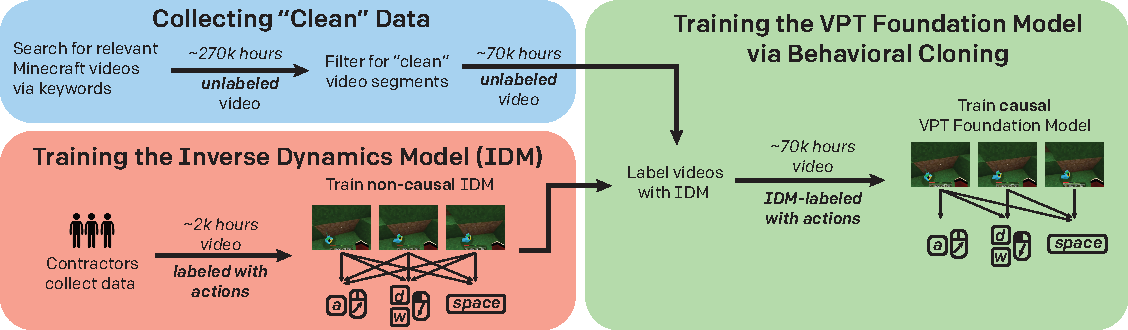
\includegraphics[width=\linewidth]{assets/vpt_method2.pdf}
\end{center}
\vspace{-10px}
\caption{Video Pretraining (VPT) Method Overview.}
\vspace{-10px}
\label{fig:method}
\end{figure}

\paragraph{Inverse Dynamics Models (IDM)} VPT, illustrated in Figure~\ref{fig:method}, requires we first collect a small amount of labeled contractor data with which to train an inverse dynamics model $p_{\textrm{\textsubscript{IDM}}}(a_t | o_{1...T})$, which seeks to minimize the negative log-likelihood of an action at timestep $t$ given a trajectory of $T$ observations $o_t~:~ t \in [1...T]$.
In contrast to an imitation learning policy, the IDM can be non-causal, meaning its prediction for $a_t$ can be a function of both past and \emph{future events}, i.e. $o_{t' > t}$.
Compared to the behavioral cloning objective of modeling the distribution of human intent given past frames only, we hypothesize that inverting environment dynamics is easier and more data efficient to learn.
Indeed, Sec.~\ref{section:results_IDM} will show that the IDM objective is much easier to learn, and furthermore Sec.~\ref{section:idm_data_scaling} will show that with very little labeled data (as few as 100 hours) we can train a fairly accurate IDM. This IDM can be used to label online videos, providing the large amount of data required for the harder task of behavioral cloning. See appendices ~\ref{appendix:training_details_IDM} and \ref{appendix:contractor_data} for IDM training and data collection details.


\paragraph{Data Filtering} We gather a large dataset of Minecraft videos by searching the web for related keywords (Appendix~\ref{appendix:collecting_internet_data}). Online videos often (1) include overlaid artifacts, such as a video feed of the player’s face, channel logos, watermarks, etc., (2) are collected from platforms other than a computer with different gameplay, or (3) are from different game modes, e.g.\ in Minecraft we only want "survival mode" where players start from scratch and must gather or craft all their items.
We call data ``clean'' if it does not contain visual artifacts and is from survival mode, and call all other data ``unclean.'' With enough data, a large enough model, and enough training compute, a BC model trained on both unclean and clean videos would likely still perform well in a clean Minecraft environment. However, for simplicity and training compute efficiency, we choose to filter out unclean segments of video (note that a video may contain both clean and unclean segments). We do this by training a model to filter out unclean segments using a small dataset (8800) of images sampled from online videos labeled by contractors as clean or unclean (Appendix~\ref{section:svm}).


\paragraph{VPT Foundation Model} We train a foundation model with standard behavioral cloning, i.e. minimizing the negative log-likelihood of actions predicted by the IDM on clean data. For a particular trajectory of length $T$ we minimize
\eqn{\min_{\theta}\sum_{t\in[1...T]}-\log\pi_{\theta}(a_t | o_1, \dots, o_t) \textrm{, where  }~ a_t\sim p_\textrm{\textsubscript{IDM}}(a_t | o_1, \dots, o_t, \dots, o_T)}
As we will see in the following sections, this model exhibits nontrivial zero-shot behavior and can be fine-tuned with both imitation learning and RL to perform even more complex skills. 
